\section{Results}

The implementation in cython, numba and c++ was run for matrix sizes n ranging from 5
to 350. Since the python version was quite slow it was only run with n in the
range of 5 to 100. All values used are average values over 5 runs.


\subsection{Number of iterations}

We will first look into the number of transformations needed to make all off
diagonal elements smaller than the tolerance level $\epsilon$, in our case
$\epsilon = 10^{-9}$, and find an estimate as a function of n, with n being the
dimension of the square matrix we are diagonalizing. In this part we will
analyze the results from the c++ implementation of Jacobis method, and compare
our results with results from the literature of between 3n$^2$ - 5n$^2$ \cite{lectures}
transformations.

To look into the n dependence \cref{fig:iterations_scaled} shows the number of
transformations scaled by n$^2$. The ratio flattens for n larger than 100. The
horisontal line shows the mean value of the ratio for n larger than 200. Using
the calculated mean value a possible equation for transformations as a function
of n is $\#transformations = 1.56\cdot n^2$.

\begin{figure}[H]
  \centering
  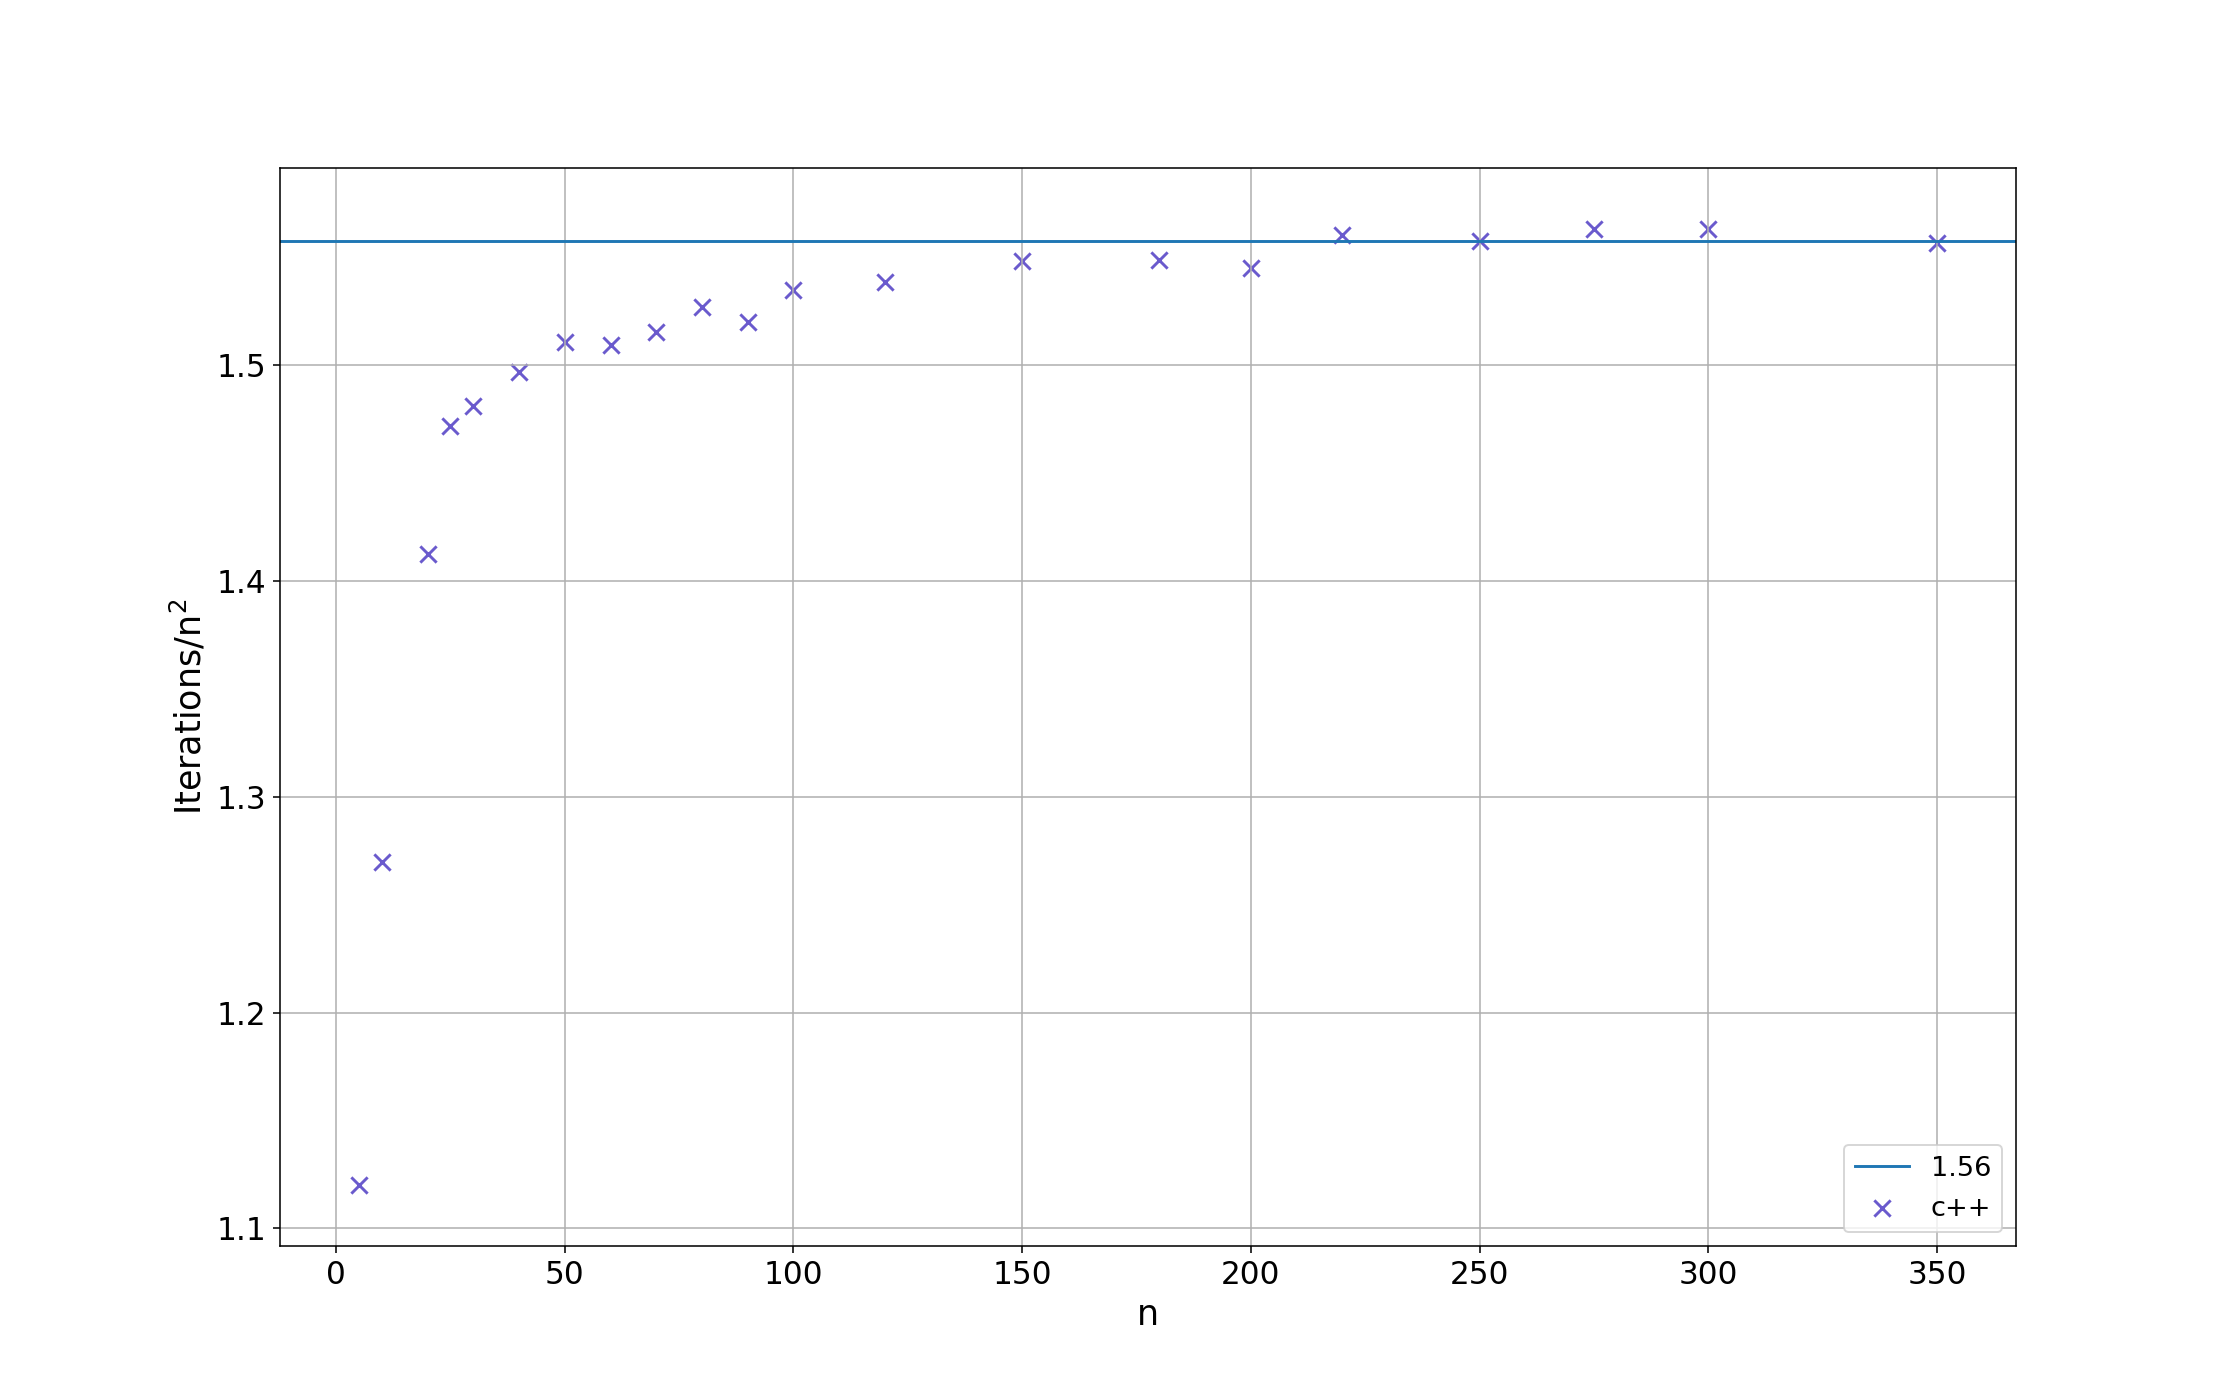
\includegraphics[width=1.0\textwidth]{../figures/iterations_compare_n2.png}
  \caption{Runs of the Jacobi method implemented in c++. Number of iterations
  needed to make all offdiagonal elements smaller than 10$^{-9}$ as function of
  matrix size n. The horisontal line shows the mean value of iterations for
  n $\geq$ 200.}

  \label{fig:iterations_scaled}
\end{figure}


\Cref{fig:iterations} shows the
actual number of transformations, our estimated relation and the values from the
literature. This seems to be a good fit to the data. Our results shows a faster
convergence than the expected values, but we are unsure of the tolerance level
that was used. If we used a lower tolerance our number of transformations would
be higher.




\begin{figure}[H]
  \centering
  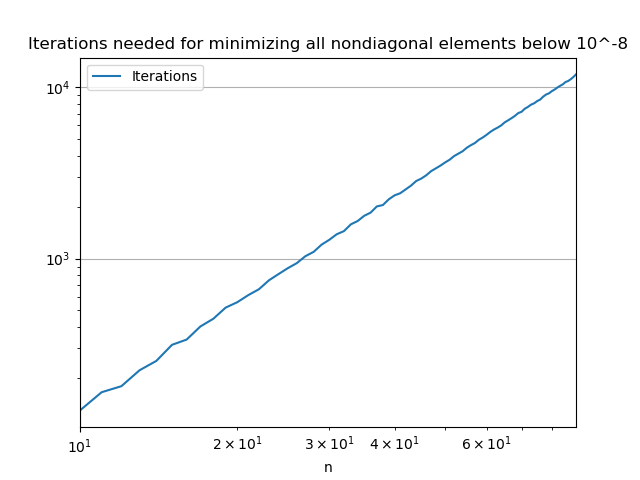
\includegraphics[width=1.0\textwidth]{../figures/iterations.png}

  \caption{Runs of the Jacobi method implemented in c++. Number of iterations
  needed to make all offdiagonal elements smaller than 10$^{-9}$ as function of
  matrix size n.}

  \label{fig:iterations}
\end{figure}


\subsection{Timing Result}

\begin{figure}[H]
  \centering
  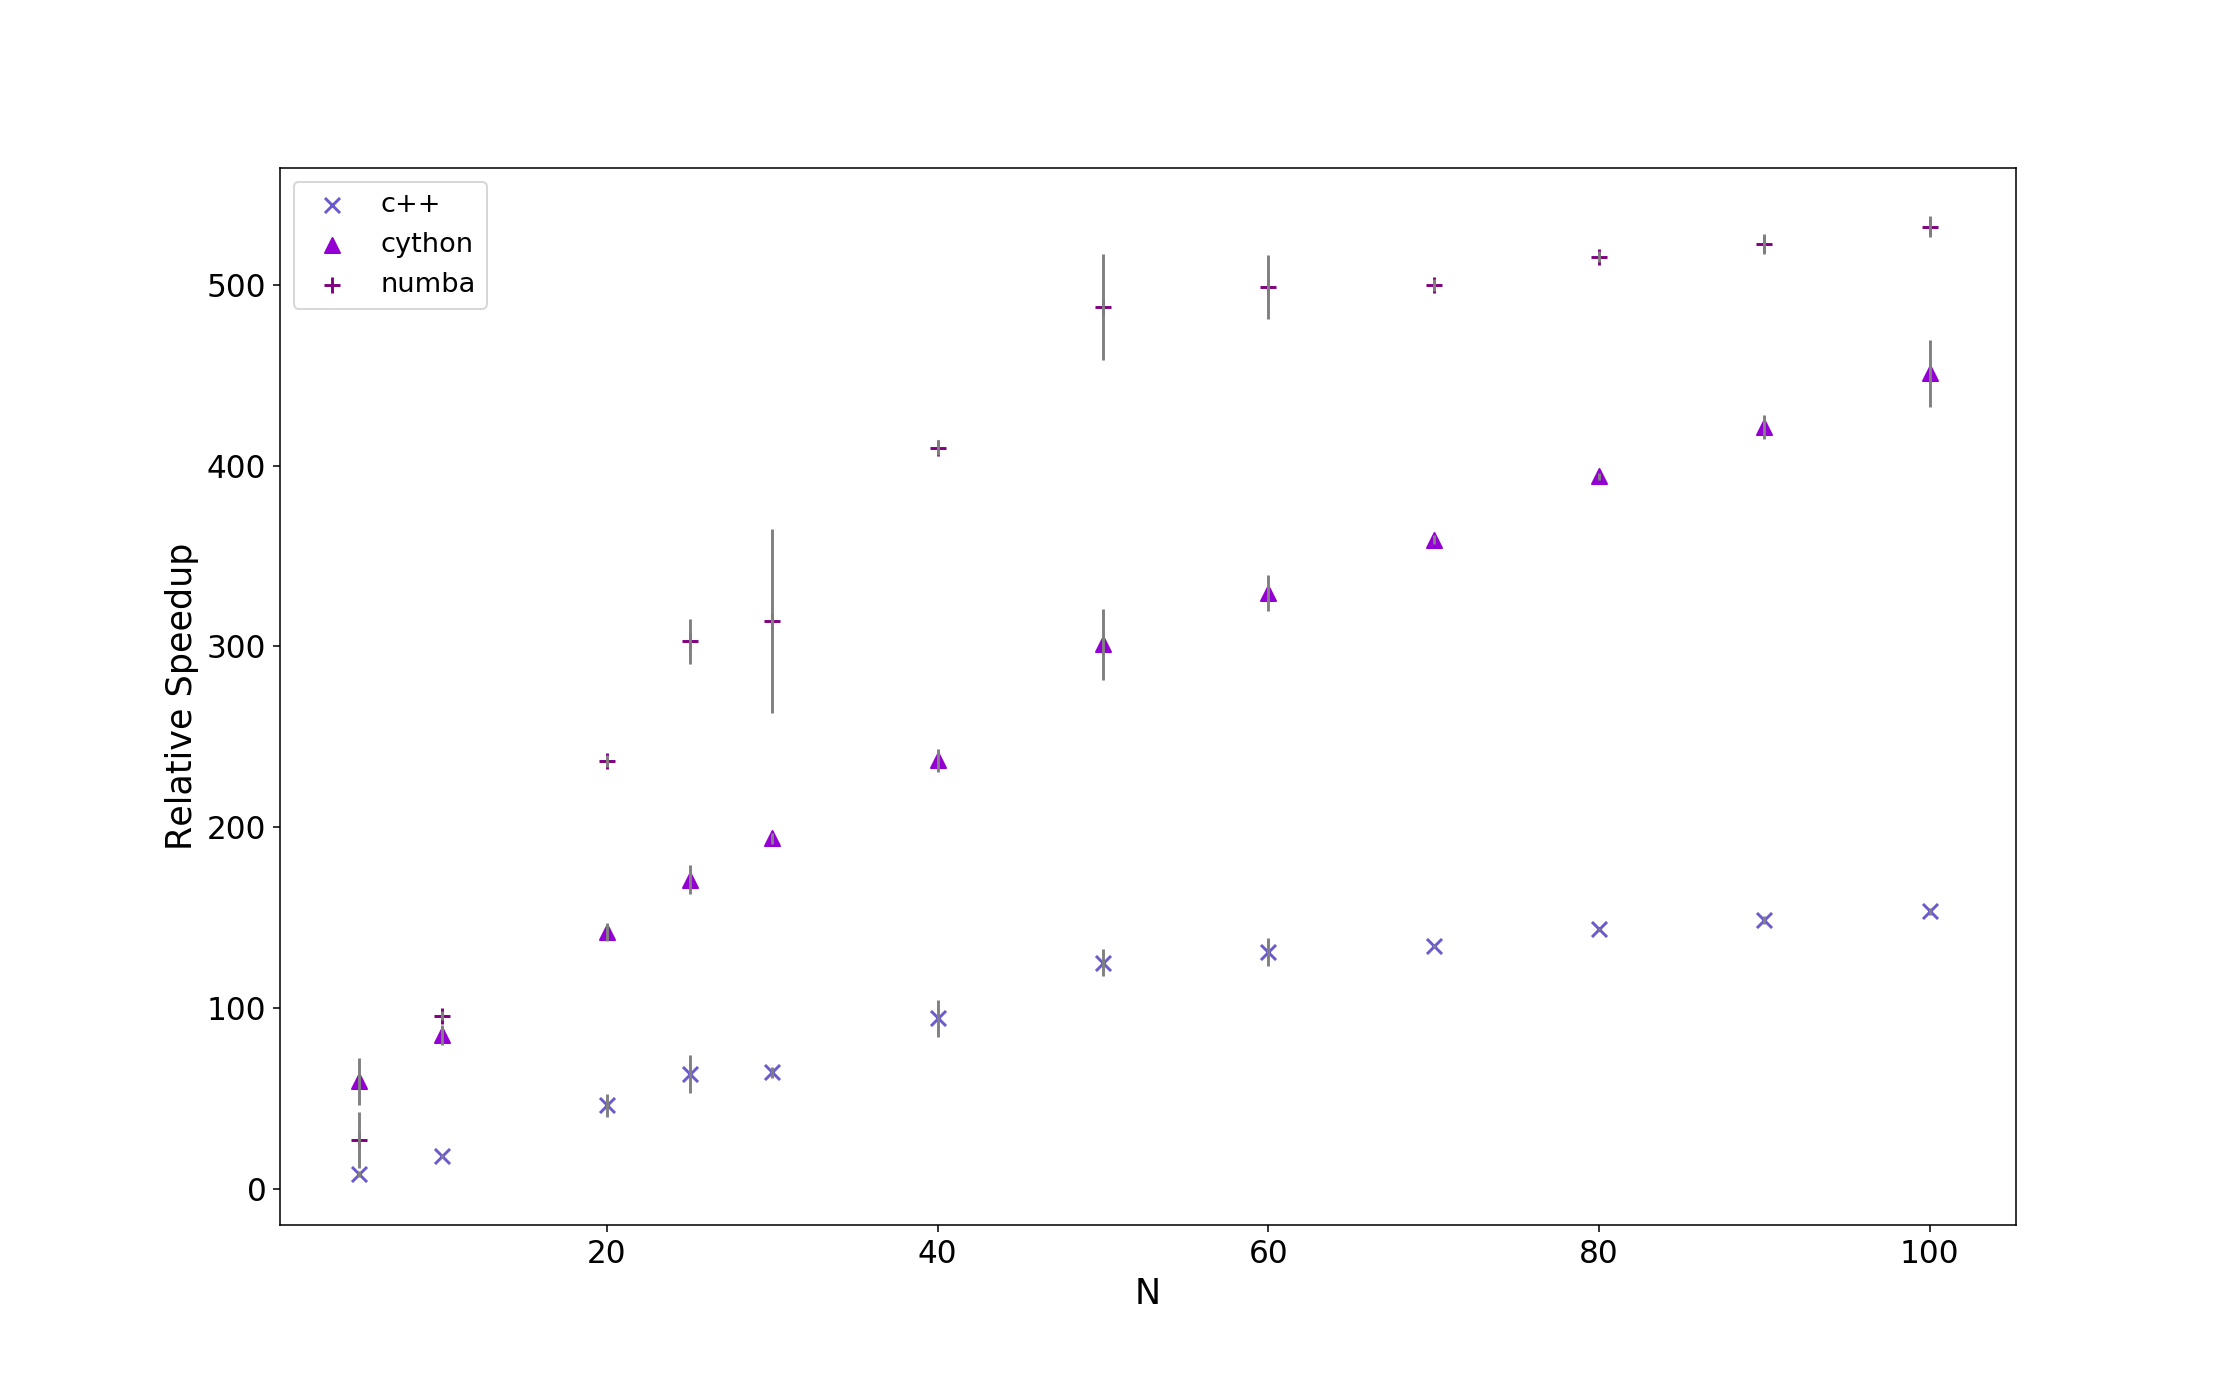
\includegraphics[width=1.0\textwidth]{../figures/avgspeed.png}
  \caption{ The average timing of 5 runs, divided by the average of the standard
  python timings. Starting from $n=5$ until $n=100$. }
  \label{fig:comp_python}
\end{figure}

\begin{figure}[H]
  \centering
  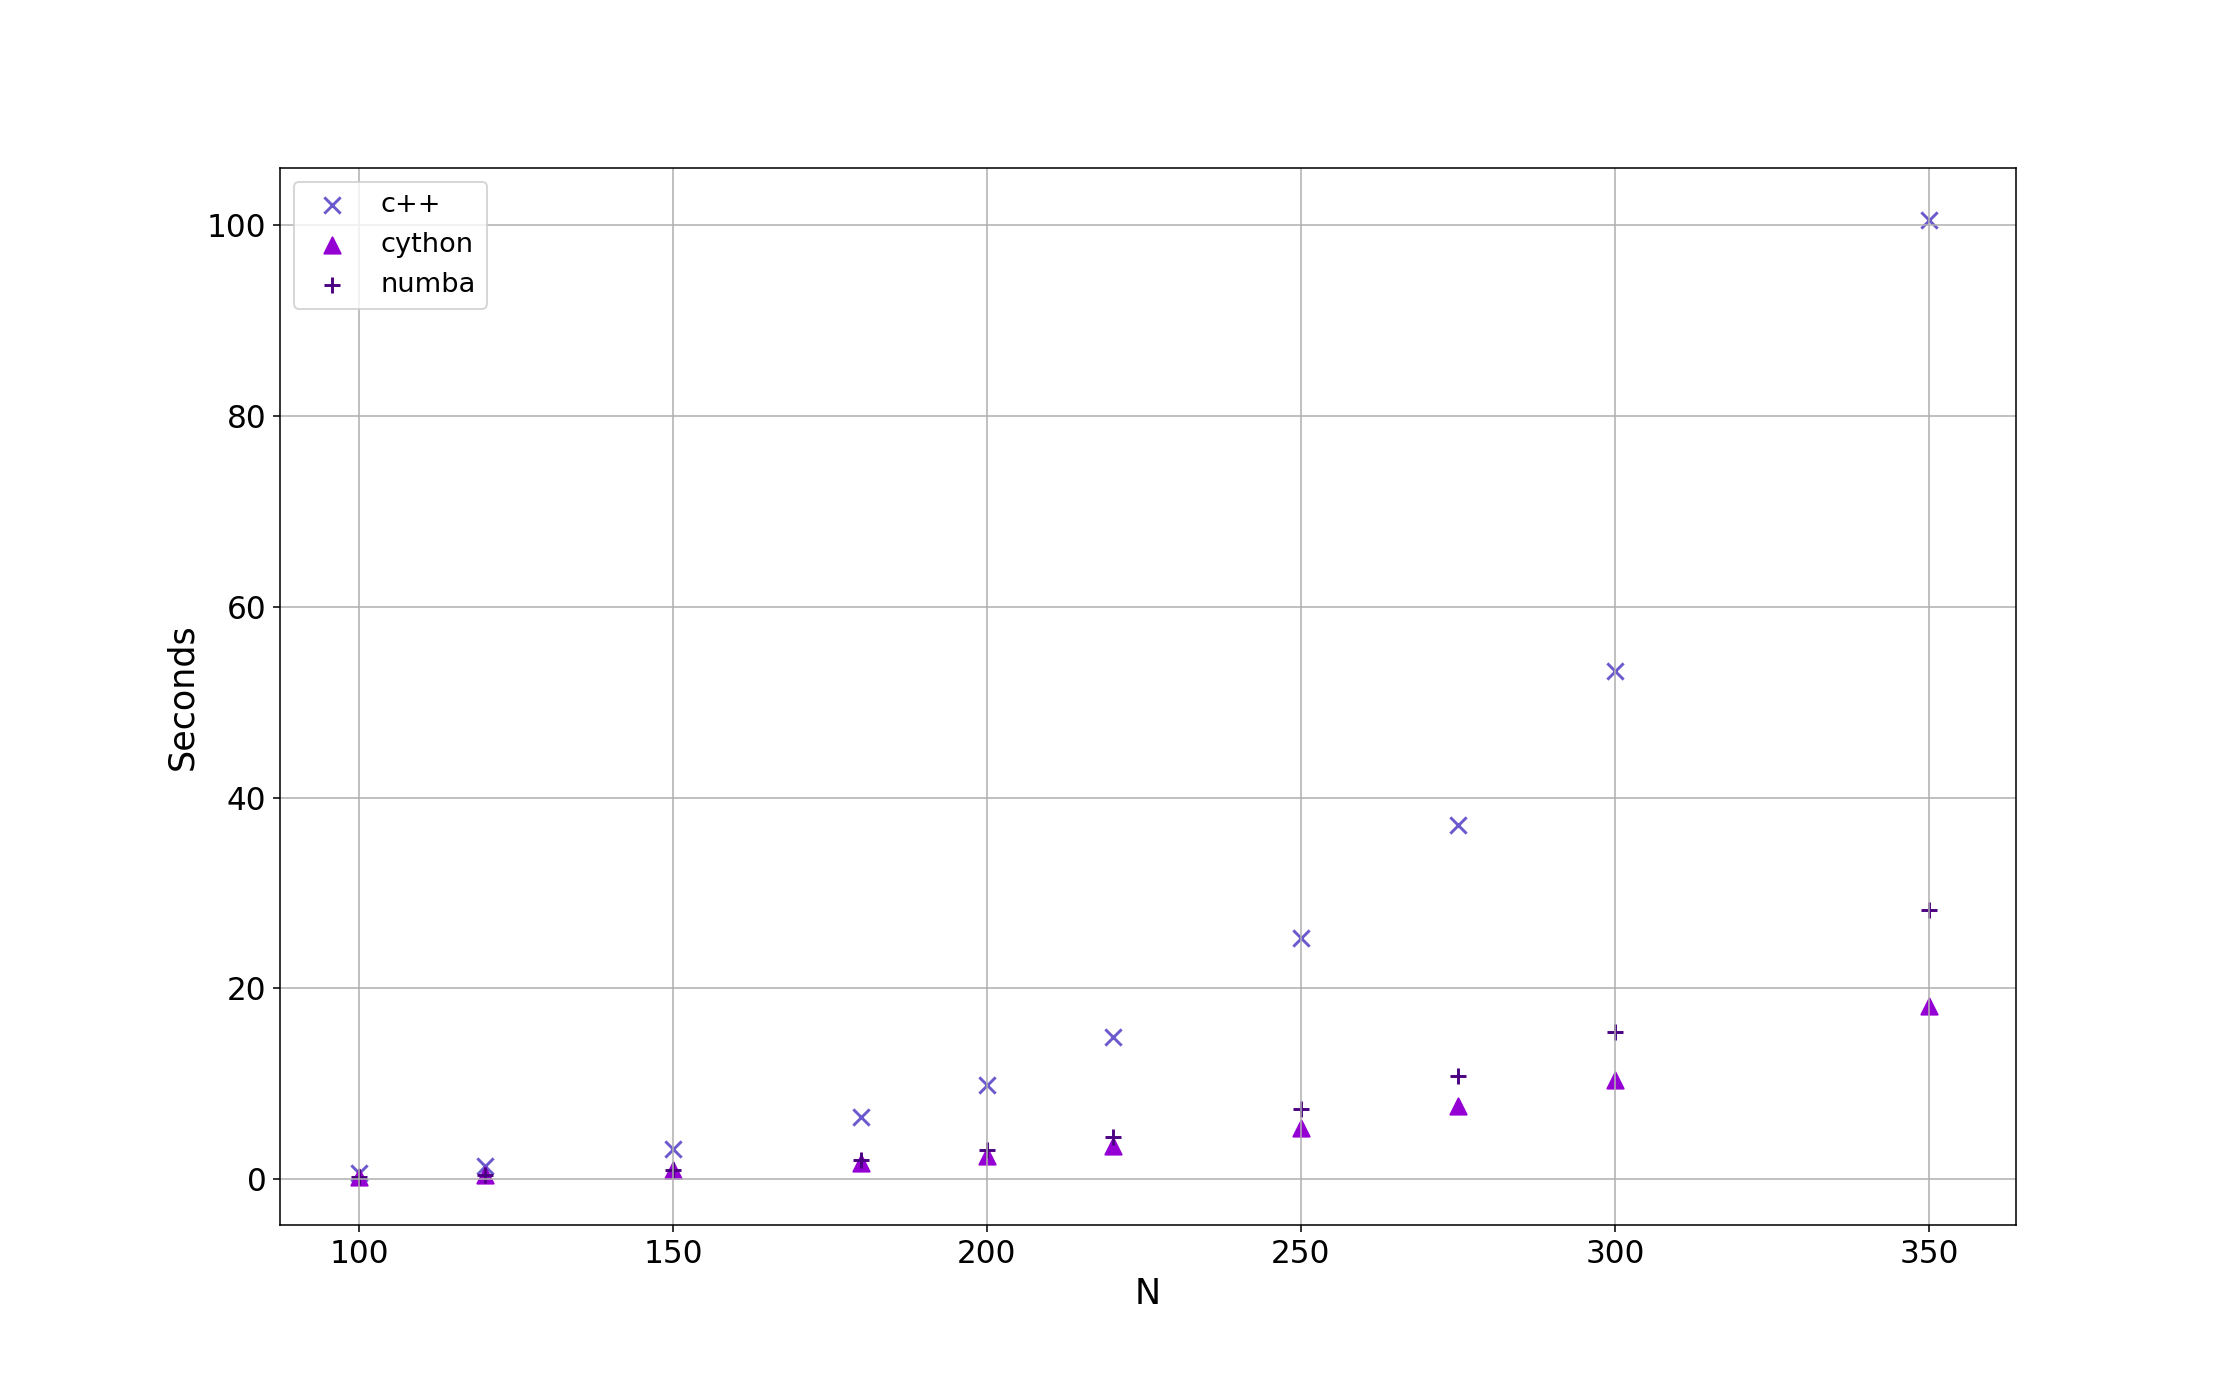
\includegraphics[width=1.0\textwidth]{../figures/speedComp_100_350.png}
  \caption{Average timing of 5 runs for the jacobi method implemented in c++, cython, numba. Starting from $n=100$ until $n=350$.}
  \label{fig:timing_largeN}
\end{figure}

\begin{figure}[H]
  \centering
  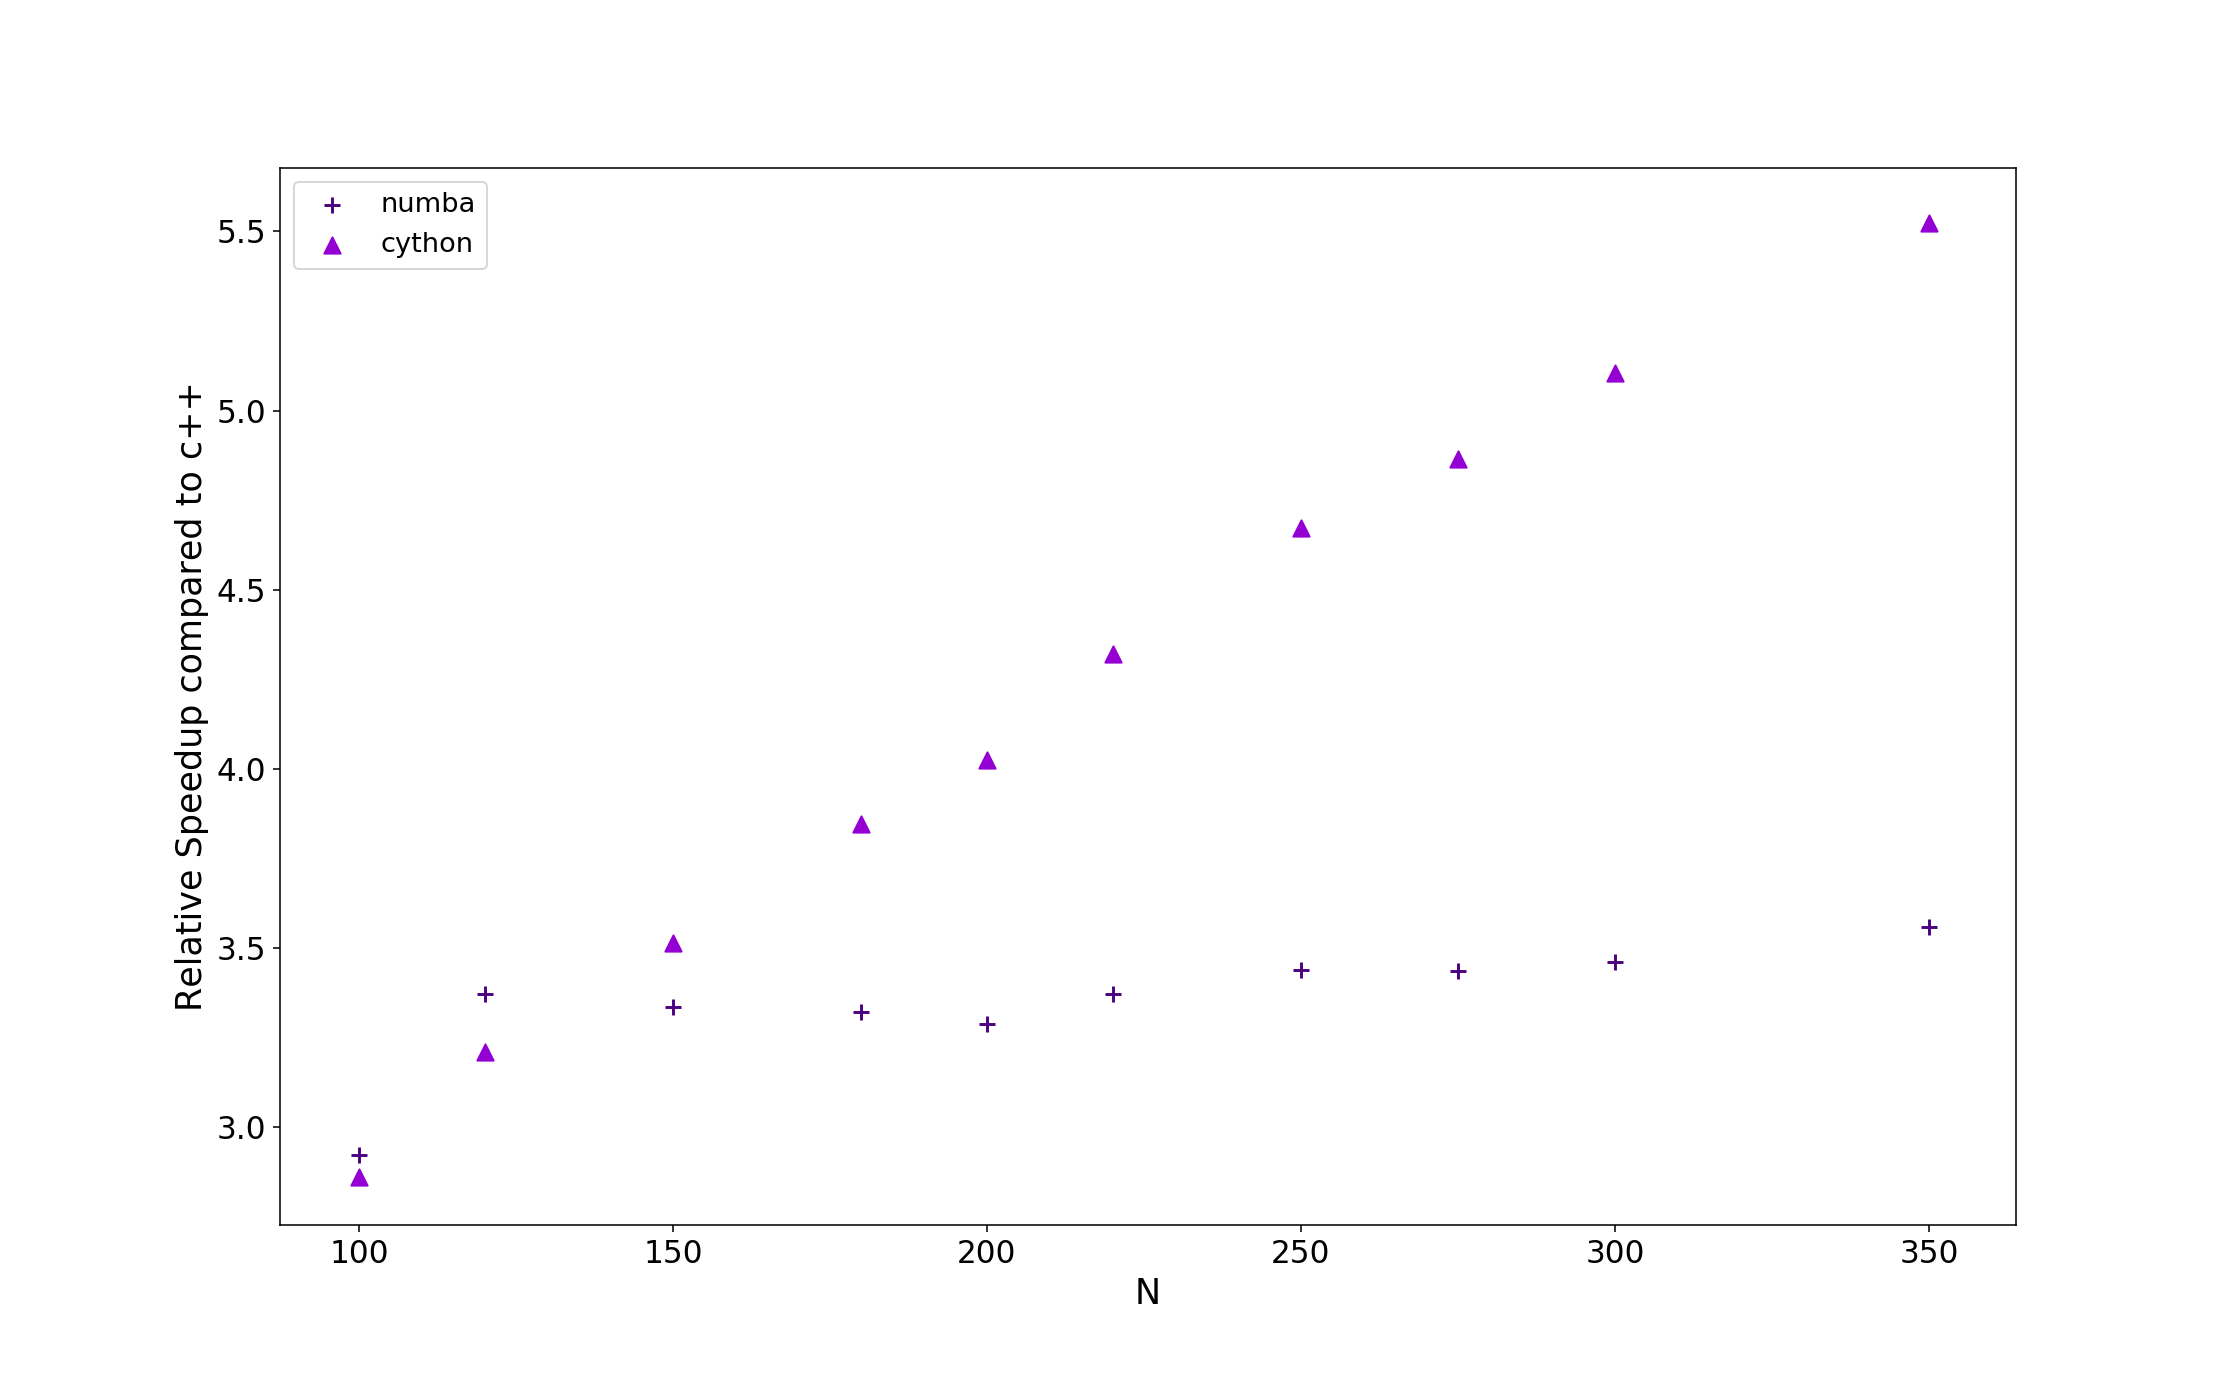
\includegraphics[width=1.0\textwidth]{../figures/speedCompC++_100_350.png}
  \caption{Relative speed up compared to c++}
  \label{fig:comp_c++}
\end{figure}
